%%%%%%%%%%%%%%%%%%%%%%%%%%%%%%%%%%%%%%%%%
% Beamer Presentation
% LaTeX Template
% Version 1.0 (10/11/12)
%
% This template has been downloaded from:
% http://www.LaTeXTemplates.com
%
% License:
% CC BY-NC-SA 3.0 (http://creativecommons.org/licenses/by-nc-sa/3.0/)
%
%%%%%%%%%%%%%%%%%%%%%%%%%%%%%%%%%%%%%%%%%

%----------------------------------------------------------------------------------------
%	PACKAGES AND THEMES
%----------------------------------------------------------------------------------------

\documentclass{beamer}

\mode<presentation> {

% The Beamer class comes with a number of default slide themes
% which change the colors and layouts of slides. Below this is a list
% of all the themes, uncomment each in turn to see what they look like.

%\usetheme{default}
%\usetheme{AnnArbor}
%\usetheme{Antibes}
%\usetheme{Bergen}
%\usetheme{Berkeley}
%\usetheme{Berlin}
%\usetheme{Boadilla}
%\usetheme{CambridgeUS}
\usetheme{Copenhagen}
%\usetheme{Darmstadt}
%\usetheme{Dresden}
%\usetheme{Frankfurt}
%\usetheme{Goettingen}
%\usetheme{Hannover}
%\usetheme{Ilmenau}
%\usetheme{JuanLesPins}
%\usetheme{Luebeck}
%\usetheme{Madrid}
%\usetheme{Malmoe}
%\usetheme{Marburg}
%\usetheme{Montpellier}
%\usetheme{PaloAlto}
%\usetheme{Pittsburgh}
%\usetheme{Rochester}
%\usetheme{Singapore}
%\usetheme{Szeged}
%\usetheme{Warsaw}

% As well as themes, the Beamer class has a number of color themes
% for any slide theme. Uncomment each of these in turn to see how it
% changes the colors of your current slide theme.

%\usecolortheme{albatross}
%\usecolortheme{beaver}
%\usecolortheme{beetle}
%\usecolortheme{crane}
%\usecolortheme{dolphin}
%\usecolortheme{dove}
%\usecolortheme{fly}
%\usecolortheme{lily}
%\usecolortheme{orchid}
%\usecolortheme{rose}
%\usecolortheme{seagull}
%\usecolortheme{seahorse}
%\usecolortheme{whale}
%\usecolortheme{wolverine}

%\setbeamertemplate{footline} % To remove the footer line in all slides uncomment this line
%\setbeamertemplate{footline}[page number] % To replace the footer line in all slides with a simple slide count uncomment this line

%\setbeamertemplate{navigation symbols}{} % To remove the navigation symbols from the bottom of all slides uncomment this line
}

\usepackage{graphicx} % Allows including images
\usepackage{booktabs} % Allows the use of \toprule, \midrule and \bottomrule in tables
\usepackage{animate}
%----------------------------------------------------------------------------------------
%	TITLE PAGE
%----------------------------------------------------------------------------------------
\title[Short title]{Volume estimation via integrating on a curve fitted point cloud} % The short title appears at the bottom of every slide, the full title is only on the title page

\author{\textbf{HiPEDS 2018 Cohort:} G. Bisbas, L. Castiglione, D. Grumberg, S. Karolčík, L. Keeble, D. Kulon, B. Kwan, C. McMeel, R. Miles, J. Ortiz, N. Perez-Nieves, V. Pham Ngoc, J. Vandebon, D. Vink} % Your name
\institute[Imperial College London] % Your institution as it will appear on the bottom of every slide, may be shorthand to save space
{ Imperial College London \\add logos % Your institution for the title page
\medskip % Your email address
}

\date{\today} % Date, can be changed to a custom date


\begin{document}

\begin{frame}
\titlepage % Print the title page as the first slide
\end{frame}



%% --------------T--H--E--O--R--Y-------------------------------------------

\begin{frame}
\frametitle{Overall structure}

\begin{itemize}
	\item  
	\item 
	\item 
	\item 
	

	
	
\end{itemize}

\end{frame}


\begin{frame}
\frametitle{The problem and the goal} 

\begin{itemize}
	\item
	
	\item 
	
\end{itemize}

\end{frame}






\begin{frame}
\frametitle{The hardware} % Table of contents slide, comment this block out to remove it
%\tableofcontents % Throughout your presentation, if you choose to use \section{} and \subsection{} commands, these will automatically be printed on this slide as an overview of your presentation

%----------------------------------------------------------------------------------------
%	PRESENTATION SLIDES
%----------------------------------------------------------------------------------------

%------------------------------------------------
 % Sections can be created in order to organize your presentation into discrete blocks, all sections and subsections are automatically printed in the table of contents as an overview of the talk
%------------------------------------------------
%\begin{figure}	
%	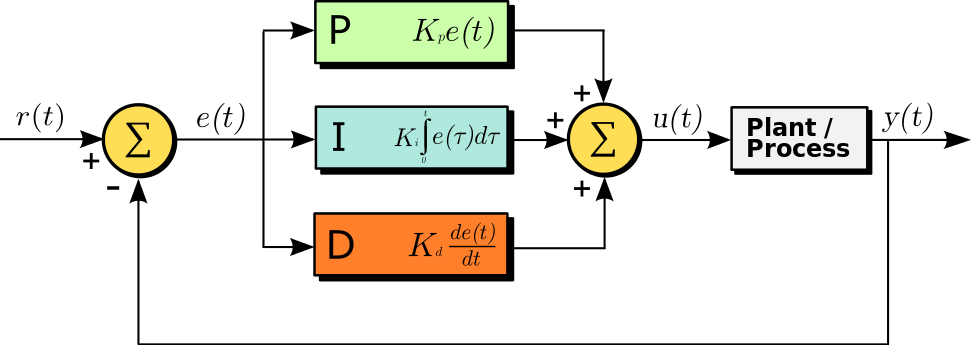
\includegraphics[width=0.8\textwidth]{Figures/PID.png}
%	\caption{PID controller}
%	\label{pid}
%\end{figure}

\begin{itemize}
	\item

	\item 
	
\end{itemize}

\end{frame}
%\subsection{Subsection Example} % A subsection can be created just before a set of slides with a common theme to further break down your presentation into chunks

\begin{frame}\frametitle{Extracting the point cloud}



\begin{itemize}
	\item 
	\item  
	\item 
\end{itemize}


\end{frame}

\begin{frame}{Denoising the point cloud}











\end{frame}


\begin{frame}{The ICP algorithm}











\end{frame}


\begin{frame}{Curve fitting with Linear Interpolation}




\end{frame}



\begin{frame}{Integration}
\begin{equation}
\iiint_V f(x,y,z) \,dx\,dy\,dz 
\end{equation}

\end{frame}


\begin{frame}{Results}

\end{frame}

\begin{frame}{References}



\end{frame}

%------------------------------------------------

%------------------------------------------------


%------------------------------------------------

\begin{frame}{Acknowledgements}
This project was proposed and supported by Royal Mail, EPSRC and Imperial College London. A special thanks to Jeremy Bradley and Ben Glocker for their support and advice throughout.
\end{frame}

%----------------------------------------------------------------------------------------

\end{document}